% !TeX root = ../main.tex
\section{Project structure}\label{sec:projectStructure}

\begin{figure}
	\centering
	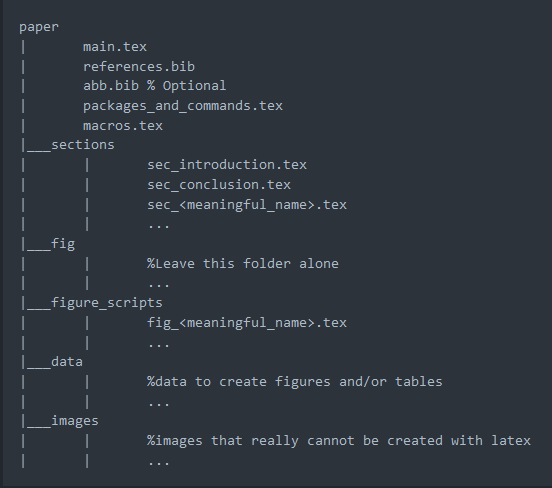
\includegraphics[width=\textwidth]{images/project_structure.png}
	\caption{The structure of the project.}
	\label{fig:projectStructure}
\end{figure}

\paragraph{Project structure}
Figure~\ref{fig:projectStructure} shows an overview of the project structure.

\why If everyone in the group follows the same structure it is easier to collaborate and you don't need to learn a new system all the time.

\paragraph{main.tex:} This is the main file of your document. Keep it as clean as possible. Conferences generally provide a template use this template to create the main file. Ideally only add the following in front of \verb|\begin{document}|:	
\verb|	|\\
\verb|	%Set to 1 to compile Figures|\\
\verb|	\def\compileFigures{0}|\\
\verb|	\newcommand{\filename}{main}|\\
\verb|	\newcounter{figureNumber}|\\
\verb|	|\\
\verb|	% !TeX root = ../main.tex
\PassOptionsToPackage{svgnames}{xcolor}
\usepackage{graphicx}
\usepackage{hyperref}

\usepackage{tcolorbox}
\tcbuselibrary{skins,breakable}
\usetikzlibrary{shadings,shadows}

\newenvironment{whyblock}[0]{%
	\tcolorbox[beamer,%
	noparskip,breakable,
	colback=LightGrey,colframe=DarkGrey,%
	colbacklower=LightGrey!75!DarkGrey,%
	title={\color{black} \large Why?}]}%
{\endtcolorbox}


\newenvironment{tipblock}[1]{%
	\tcolorbox[beamer,%
	noparskip,breakable,
	colback=LightGreen,colframe=DarkGreen,%
	colbacklower=LimeGreen!75!LightGreen,%
	title=#1]}%
{\endtcolorbox}|\\
\verb|	\newcommand{\why}{\paragraph{Why:}}|\\

	Don't write the sections in this file just use
	 \verb|\input{sections/sec_<section_name>}|.
	
	\why There will be multiple versions of your paper (submissions to different workshops, conferences, Arxiv, university events, etc.). Each requires a different template and you have to merge this template with your main.tex file. The simpler the main.tex file the better.
	
	\paragraph{package\_and\_commands.tex:} In this file you put all the \verb|\usepackage{}| imports and code for more complicated commands, which you might use in multiple projects.
	
	\why If you found a useful package or spent time creating a complicated command you want to reuse it.
	
	\paragraph{macros.tex:} This file contains all your project-specific macros. Use macros as much as possible. For example, instead of writing \verb|\mathbb{R}| every time for the real numbers create a macro \verb|\newcommand{\R}{\mathbb{R}}|. Create macros when referring to existing algorithms, data sets, and names of things. When you go through your files with Ctrl + f trying to change every instance of a declaration you decided to change the notation for, you should have created a macro for that.
	
	Why: Macros are often project specific having all of them in a small file makes it easier for collaborators to find them.
	
	\paragraph{references.bib:} The file containing all your citation references. See in the Citations section on how to create the citations.
	
	\why Keep the main.tex file clean.
	
	\paragraph{sections:} Each section of your paper should be in a separate .tex-file in this folder, give them meaningful names that start with \verb|sec_|.
	
	\why This simplifies the main file and makes it easier for people to work on different sections simultaneously.
	
	\paragraph{fig:} The figures generated by your scripts will be saved in this folder. Add everything but the .pdf-files to .gitignore.
	
	\why Compiling figures can get time-consuming and sometimes requires specific settings. People not working on the figures can just input them as .pdf See Figures for more information.
	
	\paragraph{figure\_scripts:} Each figure you create with TikZ or PGFPlots should be in a separate file with a meaningful name in this folder (starting with \verb|fig_|).
	
	\why The code to generate figures can get long and make it harder to work on the text. Outsourcing the scripts makes the files cleaner.
	
	\paragraph{data:} The data used in your graphics.
	
	\why When you rerun some experiment you only need to replace the data.
	
	\paragraph{images:} This folder contains images (e.g. .png, .jpg.) that are used in the paper. It should not contain graphics you generated somewhere else, but really only pictures.
	
	Why: Keep the main folder clean.
	
